\section{Meta-Learning}
%----------------------------------------------------------------------
%----------------------------------------------------------------------
\begin{frame}[c]{Introduction}

\notefh{Please add the visualization on the first slide for meta-learning}

\begin{itemize}
	\item Learning essentially never stops:
	\begin{itemize}
		\item Many models are periodically re-fit to track changes in the data
		\item Many models are re-fit to perform well on new tasks
	\end{itemize}
	
    \item Machine Learning is often done from scratch
    
    \item We humans do not start from scratch all the time \\ - we learned how to learn!
\end{itemize}

\end{frame}
% %----------------------------------------------------------------------
% %----------------------------------------------------------------------
% \begin{frame}[c]{Meta-Learning}
% \framesubtitle{Introduction}

% \begin{columns}
% 	\column{0.18\textwidth}
% 	Ren\'e Magritte
% 	\centering
% 	
\includegraphics[width=.9\textwidth]{w07_hpo_grey_box/images/meta_learning/magritte_1.jpg}
% 	
\includegraphics[width=.9\textwidth]{w07_hpo_grey_box/images/meta_learning/magritte_2.jpg}
% 	\column{0.258\textwidth}
% 	Francis Picabia
% 	\centering
% 	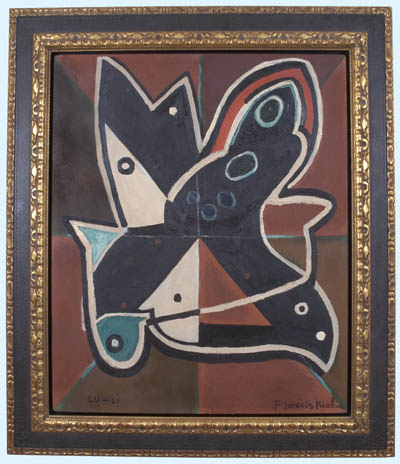
\includegraphics[width=.7\textwidth]{w07_hpo_grey_box/images/meta_learning/picabia_3.jpg}
% 	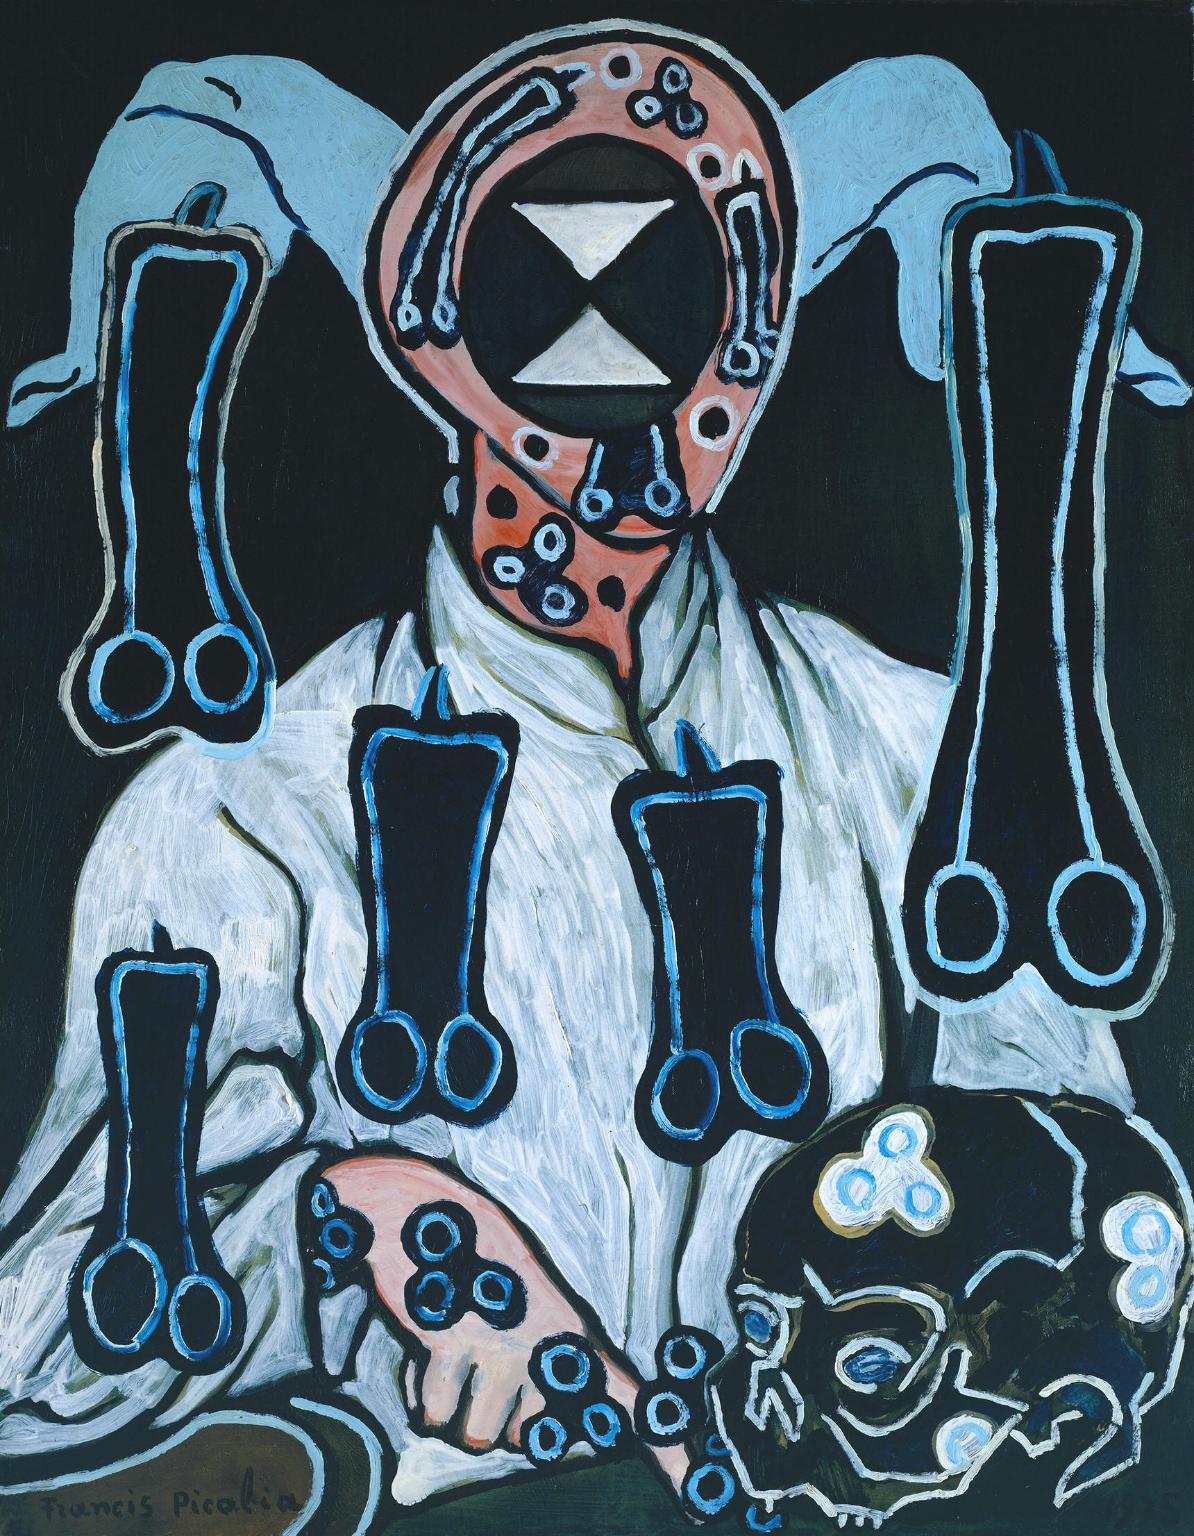
\includegraphics[width=.6\textwidth]{w07_hpo_grey_box/images/meta_learning/picabia_1.jpg}
% 	\column{0.3\textwidth}
% 	\centering
% 	Who painted that?
% 	
\includegraphics[width=.7\textwidth]{w07_hpo_grey_box/images/meta_learning/magritte_3.jpg}
	
% 	\pause
% 	Most likely most of you can identify the painter correctly, 
% 	although I presented only two pictures of each.
% \end{columns}

% \end{frame}
% % %----------------------------------------------------------------------
% % %----------------------------------------------------------------------

%----------------------------------------------------------------------
%----------------------------------------------------------------------
\begin{frame}[c]{Learning from model evaluations}

\begin{itemize}
    \item Similarly, while building ML models for a specific task, we exploit our experience with related tasks
    \item The challenge of meta-learning is to provide a systematic and data-driven approach to learn from experience 
    \item Consider that we have an access to:
        \begin{itemize}
            \item set of prior tasks: $t_{j} \in \mathcal{T}$,
            \item set of new tasks: $t_{\text{new}} \in \mathcal{T}$,
            \item set of learning algorithms, fully defined by $\theta_{i} \in \Theta$
            \item set of prior evaluations: $\dataset$, where $\dataset_{i, j} = \cost(\theta_{i}, t_{j})$
            \begin{itemize}
                \item $\dataset_{\text{new}}$ is the set of known evaluations $\cost_{i, \text{new}}$ on a new task $t_{\text{new}}$
            \end{itemize}
        \end{itemize}
    \item \emph{Goal.} Train a meta-learner using meta-data $\dataset \cup \dataset_{\text{new}}$, such that it recommends configurations for a new task better than a black-box algorithm
\end{itemize}

\hspace{11cm}\lit{\href{https://www.springer.com/gp/book/9783030053178}{AutoML Book: Chapter 2}}

\end{frame}
% %----------------------------------------------------------------------
% %----------------------------------------------------------------------

%----------------------------------------------------------------------
%----------------------------------------------------------------------
\begin{frame}[c]{Learning from task properties}

\begin{itemize}
    \item Other than characterize the data by its performance, we can extract characterizations (called \alert{meta-features}) from data at hand 
    \item Each task $t_j$ can be described by a vector of $K$ meta-features:
        \begin{equation*}
            m(t_j) = (m_{j, 1}, \dots, m_{j, K})
        \end{equation*}
    \item This vector can be used to define the similarity measure between two tasks, e.g. calculating the Euclidean distance between $m(t_i)$ and $m(t_j)$
    \item Based on similarity, we can transfer information from the most similar tasks to the new task $t_{\text{new}}$
    \end{itemize}

\hspace{11cm}\lit{\href{https://www.springer.com/gp/book/9783030053178}{AutoML Book: Chapter 2}}

\end{frame}
% %----------------------------------------------------------------------
% %----------------------------------------------------------------------

% \begin{frame}[c]{Meta-Learning}
% \framesubtitle{Supervised Learning revisited}

% Dataset:
% \begin{equation*}
% \dataset = \{(x_1, y_1), \ldots, (x_k, y_k) \}
% \end{equation*}

% \bigskip
% \pause

% Learning a model $\phi$ (e.g., weights of a neural network):
% \begin{eqnarray*}
% \argmax_{\phi} \log p(\phi|\dataset)\\
% \pause
% = \argmax_{\phi} \log p(\dataset | \phi) + \log p(\phi) \\
% \pause
% = \argmax_{\phi} \sum_i \log p(y_i | x_i, \phi) + \log p(\phi)
% \end{eqnarray*}

% \pause

% Challenge:
% \begin{itemize}
% 	\item Learning starts from scratch
% 	\item We might only have very few examples in $\dataset$ 
% \end{itemize}

% \end{frame}
% %----------------------------------------------------------------------
% %----------------------------------------------------------------------
% \begin{frame}[c]{Meta-Learning}
% \framesubtitle{Problem formulation}

% Dataset:
% \begin{equation*}
% \dataset = \{(x_1, y_1), \ldots, (x_k, y_k) \}
% \end{equation*}
% Set of datasets (meta-datasets):
% \begin{equation*}
% \mdata = \{\mathcal{D}_1, \ldots, \mathcal{D}_n, \}
% \end{equation*}

% \pause
% Can we include these meta-datasets to improve learning on $\dataset$?
% \begin{equation*}
% \argmax_{\phi} \log p(\phi|\dataset, \mdata)
% \end{equation*}

% \pause
% \medskip

% \alert{Idea:} Instead of keeping $\mdata$ forever, we want to distill the knowledge into \alert{meta-parameters $\theta$}: $p(\theta|\mdata)$
 
% \end{frame}
% %----------------------------------------------------------------------
% %----------------------------------------------------------------------
% \begin{frame}[c]{Meta-Learning}
% \framesubtitle{Problem formulation}

% In meta-learning, we want to learn:
% \begin{eqnarray*}
% \argmax_{\phi} \log p(\phi|\dataset, \mdata) \\
% \pause
% = \argmax_{\phi} \log \int_{\Theta} p(\phi \mid \dataset, \theta) p(\theta \mid \mdata) d\theta\\
% \pause
% \approx \argmax_{\phi} \log p(\phi | \dataset, \theta^*) + \log p(\theta^* | \mdata)\\
% \pause
% = \argmax_{\phi} \log p(\phi | \dataset, \theta^*)
% \end{eqnarray*}

% \pause

% \begin{center}
% \begin{minipage}{0.5\textwidth}
% \begin{block}{Meta-learning problem}
% \begin{equation*}
% \theta^* \in \argmax_{\theta} \log p(\theta | \mdata)
% \end{equation*}
% \end{block}
% \end{minipage}
% \end{center}

% \end{frame}
% %-----------------------------------------------------------------------
% %-----------------------------------------------------------------------
% \begin{frame}[c]{Meta-Learning}
% \framesubtitle{AutoML $\subset$ Meta-Learning}

% \begin{itemize}
% 	\item AutoML can be seen as a special case of meta-learning \pause
% 	\medskip
% 	\item $\theta$ could be:
% 	\begin{itemize}
% 		\item a hyperparameter configuration ($\lambda$) 
% 		\item a neural network architecture
% 	\end{itemize}
% 	\pause
% 	\medskip
% 	\item What would be $\mdata$ here? 
% 	\pause
% 	\begin{itemize}
% 		\item A dataset on which we optimized $\lambda$ (e.g. CIFAR-10)\\ such that we can use it on another dataset (e.g. imagenet)
% 	\end{itemize}
% \end{itemize}	

% \end{frame}
% %-----------------------------------------------------------------------
% %-----------------------------------------------------------------------
% \begin{frame}[c]{Meta-Learning}
% \framesubtitle{Meta-Learning $\subset$ AutoML}

% \begin{itemize}
% 	\item Meta-learning can be powerful to complement AutoML
% 	\pause
% 	\medskip
% 	\item We can learn a lot of things from $\mdata$ to improve the performance on new datasets, e.g.:
% 	\begin{itemize}
% 		\item pre-initialization of networks weights
% 		\item learning a meta-DNN to predict how to train another target-DNN	\end{itemize}
% \end{itemize}	

% \end{frame}
%-----------------------------------------------------------------------
%-----------------------------------------------------------------------
\begin{frame}[c]{Meta-Features in Machine Learning}

\begin{itemize}
	\item \alert{Simple} - easily extracted from the data, describe the basic dataset structure: e.g. number of features, patterns or classes. \pause
	
	\item \alert{Statistical} - characterize the data via descriptive statistics: e.g. average, standard deviation, correlation, the kurtosis or the dispersion of the label distribution. \pause
	
	\item \alert{Information-theoretic} - measure the class entropy in the data, capturing the amount of information in the data and their complexity. \pause 
    
    \item \alert{Model-based} - extracted from a model induced using the training data, they are often based on properties of decision tree models: e.g. the number of leaves, the number of nodes, the shape of the tree. \pause
		
	\item \alert{Landmarking} - computed by running several fast machine learning algorithms on the dataset. Based on their learning scheme they can capture different properties of the dataset, like e.g. linear separability. \pause
	
	\item \alert{Others} - not included in the previous groups, such as standalone measures, time related measures, concept and case-based measures, clustering and distance-based measures.
	
\end{itemize}

\end{frame}
%-----------------------------------------------------------------------
%-----------------------------------------------------------------------
\begin{frame}[c]{Warmstarting}
	
\begin{itemize}
	\item Recap: Instead of starting from a random configuration we often start from a expert-defined configuration for hyperparameter optimization (HPO)
	\pause
	\item We also know that such a default configuration often does not perform well on a new dataset
	\begin{itemize}
		\item Otherwise there would be no point in HPO
	\end{itemize}
	\pause
	\item \alert{Can we learn from previous datasets $\mdata$ how to initialize HPO?}\\
	(i.e., running an initial design)
%	\begin{itemize}
%		\item the same ideas also apply to NAS
%		\item for simplicity we focus on HPO 
%	\end{itemize}
\end{itemize}

\end{frame}
%-----------------------------------------------------------------------
%----------------------------------------------------------------------
%----------------------------------------------------------------------
\begin{frame}[c]{Model-Warmstarting}

\begin{itemize}
	\item Many HPO optimizers make use of some kind of a predictive model,\\
	e.g., Bayesian optimization
	\item By running HPO over and over again on different datasets,
	we can actually learn something about the search landscape
	\begin{itemize}
		\item E.g., what are bad regions of the configuration space in general
	\end{itemize}
	\smallskip
	\item Given: $n$ predictive models $\surro_{\dataset_i}: \pcs \to \mathbb{R}$ from HPO on $\dataset_{\text{meta}}$	
	\item \alert{How can we use these $\surro_{\dataset_i}$ to speed up HPO?}
\end{itemize}


\end{frame}
%-----------------------------------------------------------------------

%-----------------------------------------------------------------------
%-----------------------------------------------------------------------
\begin{frame}[c]{Task-independent Recommendations}

\begin{columns}[T] % align columns
\begin{column}{.48\textwidth}

    \only<1->{
    \begin{itemize}
        \item \emph{Idea:} learn a sorted list of defaults
        \item \emph{Method:} mostly greedy 
        \item \emph{Results:} improves over Random Search and Bayesian Optimization
    \end{itemize}}

    \only<2->{
    \begin{block}{Advantages}
    \begin{itemize}
    	\item Easy to share and use
    	\item Strong anytime performance
    	\item Embarrassingly parallel
    \end{itemize}
    \end{block}}
    
    \only<2->{
    \begin{block}{Disadvantages}
    \begin{itemize}
    	\item Not adaptive
    \end{itemize}
    \end{block}}

\end{column}%

\hfill%

\begin{column}{.48\textwidth}

    \centering
    \onslide<1->{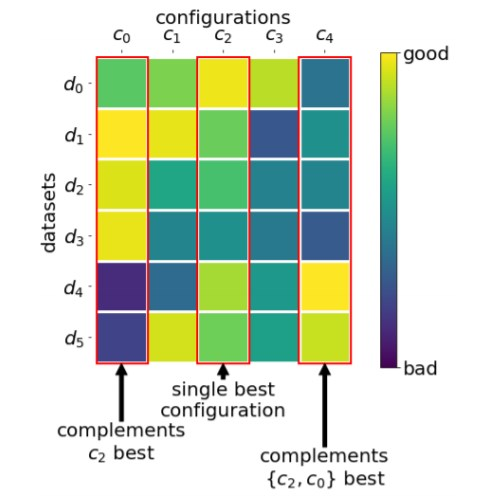
\includegraphics[width=.8\textwidth]{w07_hpo_grey_box/images/meta_learning/task_independent.jpg}}
%    \only<2->{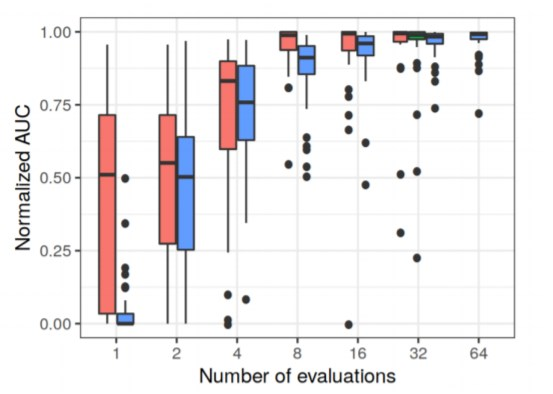
\includegraphics[width=.9\textwidth]{w07_hpo_grey_box/images/meta_learning/task_independent_results.jpg}}


\end{column}
\end{columns}  



\vspace{0.5cm}
\hspace{6cm}
\lit{\href{https://link.springer.com/article/10.1007/s10994-017-5684-y}{Wistuba et al. 2015a}}, \lit{\href{https://arxiv.org/pdf/1802.02219.pdf}{Feurer et al. 2018}},  \lit{\href{}{Pfisterer et al. 2018}}



\end{frame}
%-----------------------------------------------------------------------
%-----------------------------------------------------------------------

%-----------------------------------------------------------------------
%-----------------------------------------------------------------------
\begin{frame}[c]{Joint model for Bayesian optimization}

\begin{columns}[T] % align columns
\begin{column}{.38\textwidth}

\begin{itemize}
    \item<1-> Jointly train a „deep“ neural network on all tasks 
    \item<2-> Have a separate output layer (head) for each tasks 
    \item<3-> Each head is a Bayesian linear regression 
    \item<4-> Feature extraction on hyperparameter configurations 
    \item<5-> (Recall DNGO)
\end{itemize}
\end{column}%

\hfill%

\begin{column}{.58\textwidth}
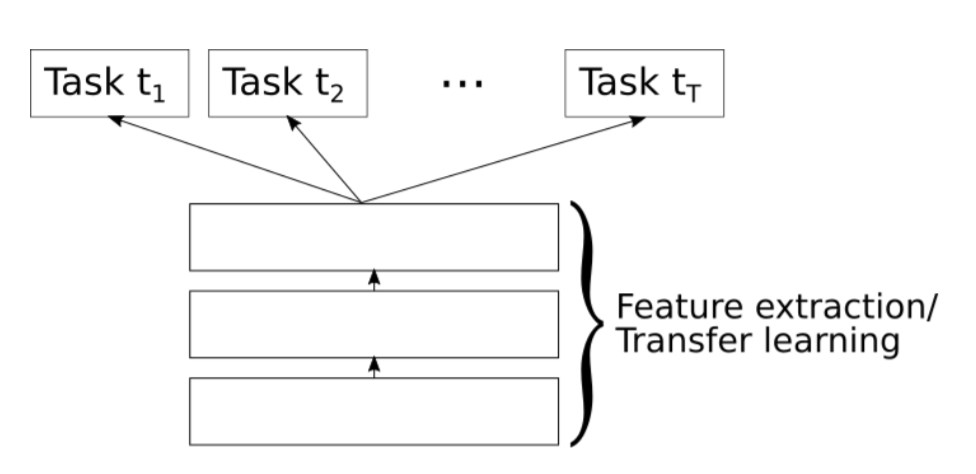
\includegraphics[width=0.9\textwidth]{w07_hpo_grey_box/images/meta_learning/perrone_int.jpg}
\end{column}%
\end{columns}

\hspace{12cm}\lit{\href{http://papers.nips.cc/paper/7917-scalable-hyperparameter-transfer-learning.pdf}{Perrone et al. 2018}}

\end{frame}
%-----------------------------------------------------------------------
%-----------------------------------------------------------------------
%\begin{frame}[c]{Joint model for Bayesian optimization}
%
%\centering
%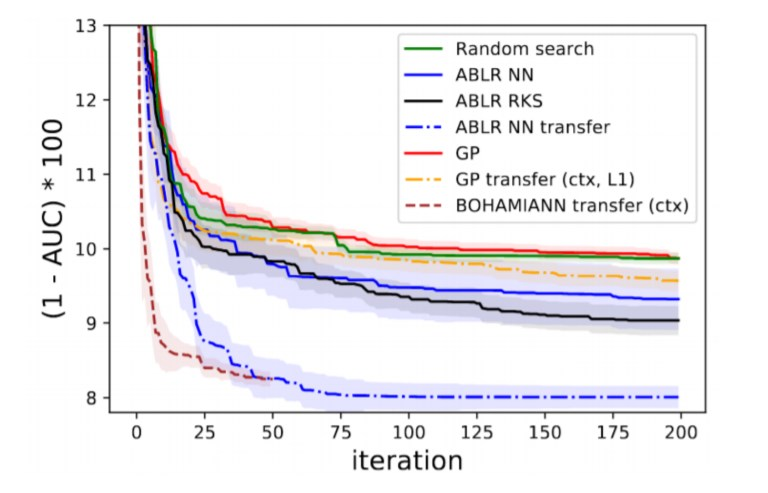
\includegraphics[width=0.7\textwidth]{w07_hpo_grey_box/images/meta_learning/perrone_res.jpg}
%
%\end{frame}
%-----------------------------------------------------------------------
%-----------------------------------------------------------------------

%----------------------------------------------------------------------
%----------------------------------------------------------------------
\begin{frame}[c]{Learning a Black-box Optimization Algorithm from Data}

\myit{

    \item Recall the black box optimization setting:
    \begin{enumerate}
        \item Given the current state of knowledge $\iter[\bocount]{h}$, propose the next query point $\iter[\bocount]{x}$
        \item Observe the response $\iter[\bocount]{y}$ \& update any internal statistics to produce $\iter[\bocount+1]{h}$
    \end{enumerate}
    
    \pause
    \bigskip
    
    \item \alert{Learning} a blackbox optimization algorithm
    \myit{
        \item Learn a mapping from $\iter[\bocount]{h}$ to next query $\iter[\bocount]{x}$
        \item This mapping can be a (recurrent) neural net $\text{NN}_{\phi}: \iter[\bocount]{h} \mapsto \iter[\bocount]{x}$ parameterized by weights $\phi$   
\pause        
        \item \alert{This mapping $\text{NN}_{\phi}$ constitutes a blackbox optimization algorithm}
        \myit{
            \item Should be learned on a \alert{meta-train} set of blackbox functions \& generalize to new functions
%            \item Like a manually-designed algorithm ...
        }

%\pause
%        \item Since $\iter[\bocount]{h}$ captures a \alert{sequence}, a recurrent NN $RNN_{\phi}:\iter[\bocount]{h} \mapsto \iter[\bocount]{x}$ makes sense

\pause
\bigskip
    
    }
    
    \item Existing approaches for learning a blackbox optimizer
    \myit{
        \item \alert{Gradient descent} on $\phi$  \lit{\href{http://proceedings.mlr.press/v70/chen17e.html}{Chen et al. 2017}}
        \myit{
            \item Simplest technique, but requires backpropagation through the optimization trace
            \item This also requires the blackbox functions $f$ used for training to be differentiable
       }
        \item \alert{Reinforcement learning} \lit{\href{https://arxiv.org/abs/1606.01885}{Li \& Malik, 2016}}
        \myit{
            \item Can be harder to get to work, but does not require differentiable $f$
        }
    
%        \item Gradient-free approaches should also work

    }
}

\end{frame}
%----------------------------------------------------------------------
%----------------------------------------------------------------------
%-----------------------------------------------------------------------
%-----------------------------------------------------------------------
\begin{frame}[c]{Learning Acquisition Functions}

\begin{itemize}
	\item Learning a complete optimization algorithm  \alert{requires a lot of data}
	\item A more \alert{sample-efficient} would be to \alert{only replace hand-designed parts} of an algorithm

\bigskip
\pause
	\item In Bayesian optimization, a critical hand-designed heuristic is the acquisition function
	\begin{itemize}
		\item Trade-off between exploitation and exploration
		\item Depending on the problem at hand, you might need a different acquisition function
		\pause
		\item Choices: PI, EI, UCB, ES, KG, \dots 
		%all of them are \alert{myopic} (no long-term look-ahead)
	\end{itemize}
\pause
\bigskip

    \item \alert{Idea:} Learn a \alert{neural acquisition function} from data, but still make use of the sample efficiency of Gaussian processes \lit{\href{https://openreview.net/forum?id=ryeYpJSKwr}{Volpp et al. 2020}}

\pause
\medskip
    \item Two options:
    \myit{
        \item Only depend on predicted mean and variance: $\acq_\theta(x) = \acq_\theta(\mu_t(x), \sigma_t(x))$ 
        \myit{
            \item This allows to learn a general acquisition function
        }
        \item Also depend on the $x$ value: $\acq_\theta(x) = \acq_\theta(\mu_t(x), \sigma_t(x), \alert{x})$  
    }

\end{itemize}


\end{frame}
%-----------------------------------------------------------------------

%-----------------------------------------------------------------------
\begin{frame}[c]{Questions to Answer for Yourself / Discuss with Friends}

\begin{itemize}
    \item \alert{Repetition.} What are the different kind of meta-features which can be used to describe machine learning datasets?
    
    \medskip

    \item \alert{Discussion.}
    \begin{itemize}
        \item How would you pick meta-features to be used in meta-learning hyperparameter optimization?
        \item What will happen with the meta-learning system if all prior tasks are dissimilar to the target task?
    \end{itemize}
\end{itemize}

\end{frame}